\documentclass[a4paper,1pt]{report}
\usepackage[utf8]{inputenc}
\usepackage[spanish]{babel}
\usepackage{amsfonts}
\usepackage{amsthm}
\usepackage{amssymb}
\usepackage{amsmath}
\usepackage{graphicx}
\usepackage{subcaption}
\usepackage{float}
\usepackage[rightcaption]{sidecap}

\newtheorem*{pbo}{Principio del Buen Ordenamiento}

\newtheorem*{pim}{Principio de Inducción Matemática}

\newtheorem*{teo}{Teorema}

\newtheorem*{cor}{Corolario}

\newtheorem*{dem}{Demostración}

\newtheorem*{dfn}{Definición}

\newtheorem*{lem}{Lema}

\newtheorem*{prp}{Propiedades}


% Title Page
\title{Conferencia 3 - Grafo Euleriano}
\author{}



\begin{document}
\maketitle

\begin{dfn}[Cadena]
Un camino $C = <v_1,v_1,...v_k>$, $k \geq 1$,  es una cadena en el grafo $G$ si todas las  aristas $\{v_i, v_{i+1}\} \in C$ son diferentes. es decir, es un camino que no repite aristas.
\end{dfn}

\begin{dfn}[Cadena cerrada]
Una cadena es cerrada si su primer y \'ultimo v\'ertice coinciden.
\end{dfn}

\begin{dfn}[Cadena de Euler]
Una cadena es de Euler si contiene todas las aristas del grafo.
\end{dfn}


\begin{SCfigure}[4][h]
    \caption{En el grafo: \\ $C = <1,2,6,7,3>$ es un ejemplo de cadena. \\ $C = <1,2,5,4,3,1>$ es un ejemplo de cadena cerrada. \\ $C = <8,3,7,6,2,5,4,3,1,2>$ es un ejemplo de Cadena de Euler.}
    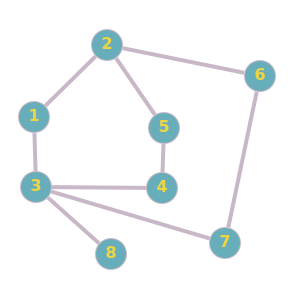
\includegraphics[width=0.2\textwidth]{figures3/Grafo.png}
    \end{SCfigure}


\begin{dfn}[Cadena Cerrada de Euler]
    Una cadena cerrada es de Euler si es una cadena de Euler cuyo primer y \'ultimo v\'ertice coinciden.
\end{dfn}

\textbf{Problema de los Siete Puentes:} En \textit{Königsberg}, ciudad de Prusia Oriental y actual ciudad rusa de Kaliningrado, el r\'io \textit{Pregolia} divid\'ia la ciudad en cuatro regiones distintas, que entonces estaban unidas mediante siete puentes. 

\begin{figure}[H]
    \centering
    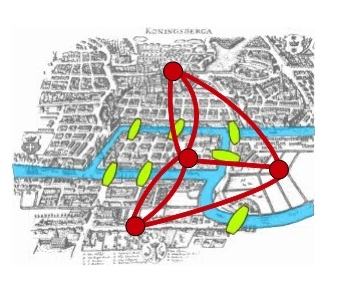
\includegraphics[width=0.4\textwidth]{figures3/puentes.jpg}
\end{figure}  


Los habitantes de la ciudad, que utilizaban los puentes como parte de su rutina diaria de transporte y ocio, inventaron un ``juego'' que consist\'ia en encontrar un recorrido para cruzar a pie toda la ciudad pasando solo una vez por cada uno de los puentes y regresando al mismo punto de inicio.  
El problema formulado en el siglo XVIII, fue resuelto por Leonhard Euler en 1736 y su resolución dió origen a la Teoría de Grafos.

\begin{dfn}[Grafo de Euler]
$G$ es un grafo de Euler (euleriano) si tiene una cadena cerrada de Euler
\end{dfn}

\begin{SCfigure}[4][h]
    \caption{Este grafo es Euleriano puesto que: \\$C =<1,2,3,4,5,2,6,7,3,1>$  \\es una cadena cerrada de Euler. \\ }
    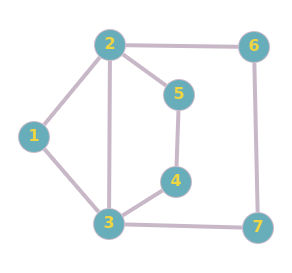
\includegraphics[width=0.3\textwidth]{figures3/GrafoEuleriano.png}
\end{SCfigure}


\begin{teo}
Sea $G$ un multigrafo conexo, se cumple que:
\begin{enumerate}
    \item $G$ es euleriano $\Leftrightarrow $ todos los v\'ertices de $G$ tienen grado par.
    \item $G$ tiene una cadena de Euler $\Leftrightarrow$ contie exactamente $2$ v\'ertices de grado impar.
\end{enumerate}
\end{teo}

\begin{dem}[Demostraci\'on propiedad $1 \Rightarrow$] Si un Grafo es euleriano entonces todos los v\'ertices tienen grado par.\end{dem}

Como $G$ es euleriano, sea $C$ la cadena cerrada de Euler que posee. 
En el recorrido de $C$ se tiene que entrar y salir de cada v\'ertice $v_i$, y cada vez que esto pasa sabemos que se est\'an analizando aristas diferentes que inciden sobre $v_i$ porque en una cadena no se repiten aristas. 
Luego para cada v\'ertice le sumamos $2$ a su grado cada vez que aparezca en la cadena, como adem\'as sabemos que todas las aristas del grafo est\'an en la cadena, al recorrer la cadena entera todos los v\'ertices tienen asignado su grado correctamente (no hay ning\'un vertice para el cual no se haya tenido en cuenta la incidencia de alguna arista) que es par $\blacksquare$.

\begin{dem}[Demostraci\'on propiedad $1 \Leftarrow$] Si todos los v\'ertices de $G$ tienen grado par entonces $G$ es euleriano.\end{dem}

Para demostrar esta implicaci\'on, nos apoyamos en el siguiente \textbf{lema:}
\begin{itemize}
    \item[] \begin{lem}
        Sea $G$ conexo, tal que todos sus v\'ertices tienen grado par, toda cadena maximal de $G$ es cerrada.
        \end{lem}
    \item[] \begin{dem}[Demostración del lema por Reducci\'on al Absurdo]\end{dem}
    Supongamos que no se cumple esta propiedad en algun grafo $G$ conexo cuyos v\'ertices todos son de grado par. 
    Sea $C = <v_1,v_2,...,v_k>$ cadena maximal de $G$ que no es cerrada, tomemos el v\'ertice $v_1$ que es uno de los extremos de la cadena, para este v\'ertice se cumple que por cada vez que aparece en medio de la cadena (sin contar la vez que aparece en el extremo), se cuentan 2 de sus aristas, por la que se llega a \'el y por la que se sale de \'el, luego si $v_1$ aparece $p$ veces como v\'ertice intermedio en $C$, se analizaron $2p$ de las aristas incidentes en $v_1$; adem\'as se tiene que en $v_1$ incide la arista que lo conecta al extremo de la cadena. Por este motivo, en $C$ se analizan $2p +1$ de las aristas que inciden en $v_1$. Como el grado de $v_1$ es par, y se han analizado una cantidad impar de sus aristas, entonces podemos decir que hay al menos una arista de $v_1$ que no pertenece a $C$, sea esa arista $\{v_0, v_1\}$, entonces $C' = \{v_0, v_1\} + C $ es una cadena que se puede construir a partir de $C$ que tiene mayor tama\~no, esto contradice el hecho de que $C$ es maximal $\blacksquare$.
    
\end{itemize}

Luego, sea $G$ conexo con todos sus v\'ertices de grado par. Sea $C$ la mayor cadena cerrada de $G$ (Sabemos que existe una cadena cerrada por el lema anterior, entonces del conjunto de cadenas cerradas tomamos la mayor), $C$ tiene que tener todas las aristas del grafo. \\

Supongamos lo contrario, entonces quedan aristas del grafo que no est\'an contenidas en $C$. \\ 

Sea $G' = G -C$ el grafo resultante de quitar las aristas de la cadena $C$ del grafo $G$. En $G'$ todos los v\'ertices tienen grado par, puesto que a cada v\'ertice del ciclo se le quitaron solo las aristas pertenecientes al ciclo que es un n\'umero par (por cada aparici\'on del v\'ertice en el ciclo se quita la arista por la que se entra y por la que se sale del v\'ertice). \\

Como asumimos que $C$ no conten\'ia todas las aristas del grafo, entonces en $G'$ hay al menos una componente conexa en la que hay aristas, en esa componente conexa como cumple que todos sus v\'ertices son de grado par, por el lema anterior cualquier cadena maximal en esa CC es cerrada, y adem\'as alguno de los v\'ertices de esta CC tiene que estar en la cadena $C$, puesto que $G$ era inicialmente conexo. \\

\begin{figure}[H]
    \centering
    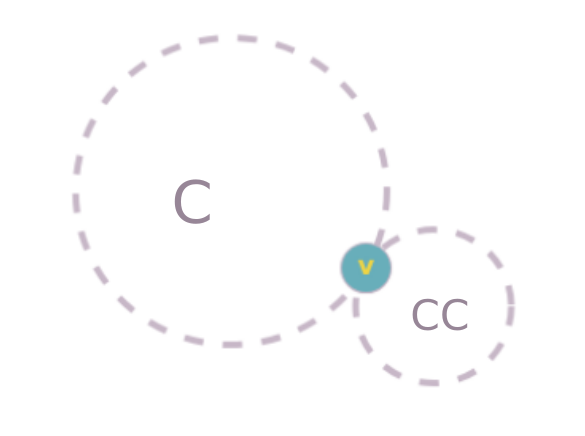
\includegraphics[width=0.4\textwidth]{figures3/Cadena+CC.png}
\end{figure}  

Sea $v_i$ uno de los v\'ertices de la CC que est\'a presente en $C$, entonces sea $C' = <x_1, x_2, ..., v_i, ..., x_k, x_1>$ una cadena maximal de la CC que contiene a $v_i$, en el grafo $G$ esta cadena $C'$ existe y como $C = <v_1, v_2,..., v_i, ..., v_t, v_1>$, es posible unir estas dos cadenas cerradas a partir de $v_i$ obteni\'endose la cadena cerrada $C'' = <v_1, v_2, ..., v_i, x_{i + 1}, ..., x_k, x_1, x_2, ...., v_i, v_{i+1}, ..., v_t, v_1>$ la cual es mayor que $C$, lo cual es una contradicci\'on puesto que $C$ es la mayor cadena cerrada de $G$, de donde se concluye que la mayor cadena cerrada de $G$ es euleriana $\blacksquare$.

\begin{dem}[Demostraci\'on propiedad $2 \Rightarrow$] Si $G$ contiene una cadena de Euler entonces tiene exactamente $2$ v\'ertices de grado impar.\end{dem}

Sea $C = <v_1, v_2,..., v_k>$ la cadena de Euler del grafo $G$, agreguemos un v\'ertice ficticio $v$ y lo conectamos a $v_1$ y a $v_k$, as\'i se forma una cadena cerrada de Euler. Como en esa cadena est\'an presentes todas las aristas, y a cada v\'ertice se entra y de cada v\'ertice se sale, se cuentan dos aristas por cada aparici\'on de un v\'ertice, de donde todos los v\'ertices tienen grado par. Luego al remover el v\'ertice ficticio $v$ y las aristas $\{v, v_1\}$ y $\{v, v_k\}$ los \'unicos v\'ertices a los cuales se les modifica el grado son $v_1$ y $v_k$, que disminuye en $1$ y pasan a tener grado impar, siendo estos dos v\'ertices los \'unicos con grado impar en $G$ y los restantes tienen grado par $\blacksquare$.

\begin{figure}[H]
    \centering
    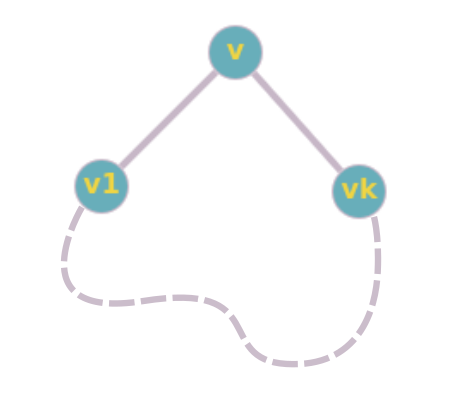
\includegraphics[width=0.3\textwidth]{figures3/Camono+v.png}
\end{figure}  

\begin{dem}[Demostraci\'on propiedad $2 \Leftarrow$] Si $G$ tiene exactamente $2$ v\'ertices de grado impar entonces contiene una cadena de Euler.\end{dem}

Sean $v_i$ y $v_j$ los dos v\'ertices de grado impar, le agregamos a $G$ el v\'ertice ficticio $v$ y las aristas $\{v, v_i\}$ y $\{v, v_j\}$, luego en el grafo tras esta modificaci\'on todos los v\'ertices tienen grado par, puesto que $v$ tiene grado $2$, a $v_i$ y $v_j$ se les agreg\'o una arista a cada uno cambiando su paridad y los restantes v\'ertices no se modificaron; por el teorema anteriormente demostrado, este grafo es euleriano, es decir que existe una cadena cerrada de Euler. Tomando esa cadena y removiendo el v\'ertice $v$ con sus dos aristas, nos queda una cadena de Euler donde sus extremos son $v_i$ y $v_j$ $\blacksquare$.

\begin{teo}
Sea $G$ un grafo con exactamente $2k$ v\'ertices de grado impar $\Rightarrow$ las aristas de $G$ se pueden particionar en $k$ cadenas disjuntas y este es el m\'inimo (siempre se puede descomponer en $k$).
\end{teo}

\begin{dem}[Demostraci\'on de que se necesitan al menos $k$ cadenas para particionar las aristas del grafo]\end{dem}

Sea $v \in V(G)$, tal que $deg(v)$ impar, entonces $v$ debe ser v\'ertice extremo de alguna cadena. N\'otese que $v$ no puede siempre estar en el medio porque cada vez que aparece en el medio de alguna cadena se cuentan dos de sus aristas y como tiene grado impar faltar\'ia una de sus aristas por estar en alguna cadena. 
Luego como cada cadena abierta tiene a lo sumo $2$ v\'ertices de grado impar, uno por cada extremo, y el grafo tiene $2k$ v\'ertices de grado impar, entonces, siempre se requieren $k$ o m\'as cadenas para particionar las aristas del grafo. 

\begin{dem}[Demostraci\'on de que $k$ cadenas es el m\'inimo]\end{dem}

Para demostrar que el m\'inimo de cadenas es $k$ (esto quiere decir que siempre hay una forma de descomponerlo en $k$ cadenas) vamos a hacer una inducci\'on en el n\'umero de parejas de v\'ertices de grado impar.

\textbf{Caso base $k =1$:} Si un grafo conexo tiene exactamente una pareja de v\'ertices de grado impar, por el teorema anterior sabemos que en este grafo hay una cadena de Euler, por tanto, se puede obtener una cadena. \\

\textbf{Hip\'otesis $k$:} Supongamos que para todo grafo conexo donde existen exactamente $2k$ v\'ertices de grado impar es posible particionar sus aristas en $k$ cadenas.\\

\textbf{Demostración $k+1$:} Sea $G$ un grafo conexo de $2k + 2$ v\'ertices de grado impar, si le agregamos al grafo un v\'ertice ficticio $v$ y lo conectamos a dos de los v\'ertices de grado impar, tendr\'iamos un grafo $G' = G + \{v\} + \{e_1, e_2\} $ donde $e_1, e_2$ son las aristas agregadas, en $G'$ existen exactamente $2k$ v\'ertices de grado impar, luego se le aplica la hip\'otesis de inducci\'on, $G'$ se puede descomponer en $k$ cadenas. 
N\'otese que en estas $k$ cadenas cada uno de los extremos tiene que ser uno de los v\'ertices de grado impar, puesto que ellos obligatoriamente tienen que aparecer alguna vez como extremo de una cadena y hay exactamente $2k$ vertices impares para $2k$ extremos de cadena. Luego el v\'ertice $v$ tiene que estar en el medio de alguna cadena, al quitarlo a \'el junto a las aristas $e_1$ y $e_2$ se incrementa en $1$ el n\'umero de cadenas, obteni\'endose las $k+1$ cadenas resultantes del grafo $G \blacksquare$. 

\end{document} 